%%% ----------
\section{Программа <<АВАНТ-конфигуратор>>}	\label{sec:configurator}

Просмотр содержимого журналов данных, просмотр текущего состояния, просмотр и изменение параметров, изменение режима работы приемопередатчика осуществляется с помощью персонального компьютера (ПК) с установленной специализированной программой <<АВАНТ-конфигуратор>> (далее конфигуратор).  Конфигуратор состоит из нескольких страниц, между которыми можно свободно переключаться в ходе работы с программой. Доступны следующие страницы:
\begin{list}{--}{}
\item настройки подключения;
\item текущее состояние;
\item общие параметры;
\item параметры защиты;
\item журналы;
\item осциллограммы.
\end{list}

	
%%% ----------
\subsection{Страница <<Настройки подключения>>}	\label{ssec:configurator_connect}

После запуска программы при подключенном к приемопередатчику ПК, конфигуратор автоматически устанавливает связь с устройством. 

Разорвать и вновь установить связь с приемопередатчиком возможно вручную с помощью кнопки <<Установить соединени>> на панели <<Соединение>>, предварительно выбрав COM-порт, к которому подключен приемопередатчик. 

Вариант исполнения приемопередатчика представлен на панели <<Исполнение>>. 
	
\begin{figure}[H]
	\center{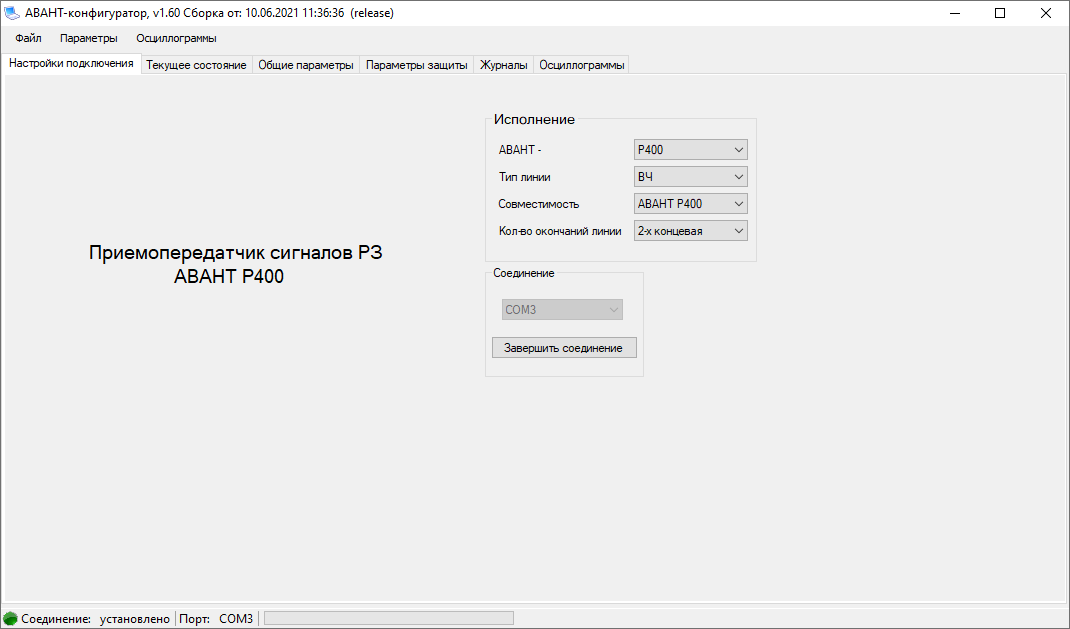
\includegraphics[width=0.8\linewidth]{configurator_connect.png}}
	
	\caption{Страница <<Настройки подключения>>}
	\label{fig:configurator_connect}
\end{figure}	
	
	
%%% ----------
\subsection{Страница <<Текущее состояние>>}	\label{ssec:configurator_state}
	
На странице <<Текущее состояние>> в режиме реального времени отображаются режим работы, текущее состояние, информация о наличии неисправностей приемопередатчика. Также на странице представлена информация об измеряемых параметрах.

\begin{figure}[H]
	\center{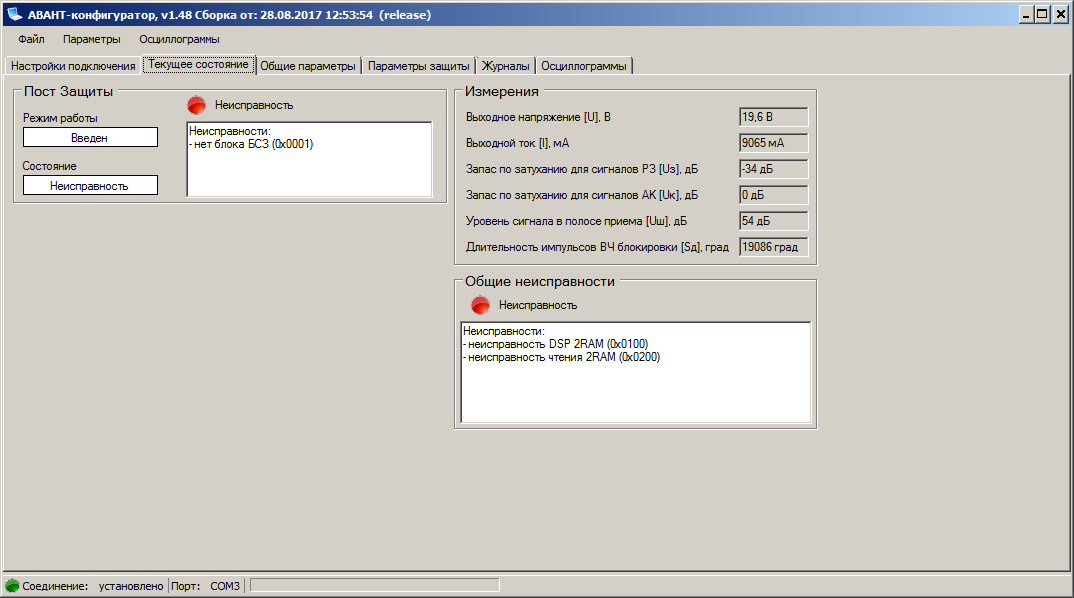
\includegraphics[width=0.8\linewidth]{configurator_state.png}}
	
	\caption{Страница <<Текущее состояние>>}
	\label{fig:configurator_state}
\end{figure}


%%% ----------
\subsection{Страница <<Общие параметры>>}	\label{ssec:configurator_param_glb}

На странице <<Общие параметры>> в режиме реального времени отображается режим работы приемопередатчика. На странице возможно изменение режима, изменение текущей даты и времени приемопередатчика, чтение, изменение и запись общих параметров работы приемопередатчика.

Запись параметров осуществляется только в режиме <<Выведен>>. 
\newline

\textbf{Изменение режима}

Для изменения режима работы приемопередатчика необходимо на панели <<Изменить режим работы>> выбрать один из предложенных режимов и нажать на кнопку <<Изменить>>, после чего необходимо ввести пароль.
\newline

\textbf{Просмотр и изменение общих параметров}

Для того чтобы просмотреть установленные в настоящее время параметры работы приемопередатчика необходимо на панели меню выбрать <<Параметры/Чтение из устройства/Общие параметры>>. Считанные из приемопередатчика параметры отобразятся в соответствующих полях панели <<Общие параметры>>.

Для того чтобы изменить параметры необходимо ввести желаемые значения параметров и на панели меню выбрать <<Параметры/Запись в устройство/Общие параметры>>.
\newline

\textbf{Сохранение и чтение общих параметров из файла}

Существует возможность сохранить измененные параметры работы приемопередатчика в файл, для этого необходимо на панели меню выбрать <<Параметры/Сохранить в файл>>, в появившемся окне выбрать место для сохранения, ввести имя файла и нажать <<Сохранить>>. В созданный файл будут сохранены все параметры работы приемопередатчика: общие и параметры защиты.

Для того чтобы считать ранее сохраненные параметры из файла необходимо на панели меню выбрать <<Параметры/Загрузить из файла>>, в появившемся окне выбрать файл с параметрами и нажать <<Открыть>>. Из выбранного файла будут считаны все параметры работы приемопередатчика: общие и параметры защиты. 
\newline

\textbf{Изменение значения даты и времени часов приемопередатчика}

Для изменения значения даты и времени часов приемопередатчика можно воспользоваться кнопкой <<Синхронизировать время с ПК>>, при этом дата и время в приемопередатчике установятся равными дате и времени подключенного ПК. Существует возможность установки часов вручную, для этого необходимо нажать на кнопку <<Установить время вручную>>, поля текущего времени и даты станут доступными для изменения, название кнопки изменится на <<Записать время в устройство>>. После чего необходимо ввести желаемые дату и время, нажать на кнопку <<Записать время в устройство>>. Название кнопки вновь изменится на <<Установить время вручную>>. 

\begin{figure}[H]
	\center{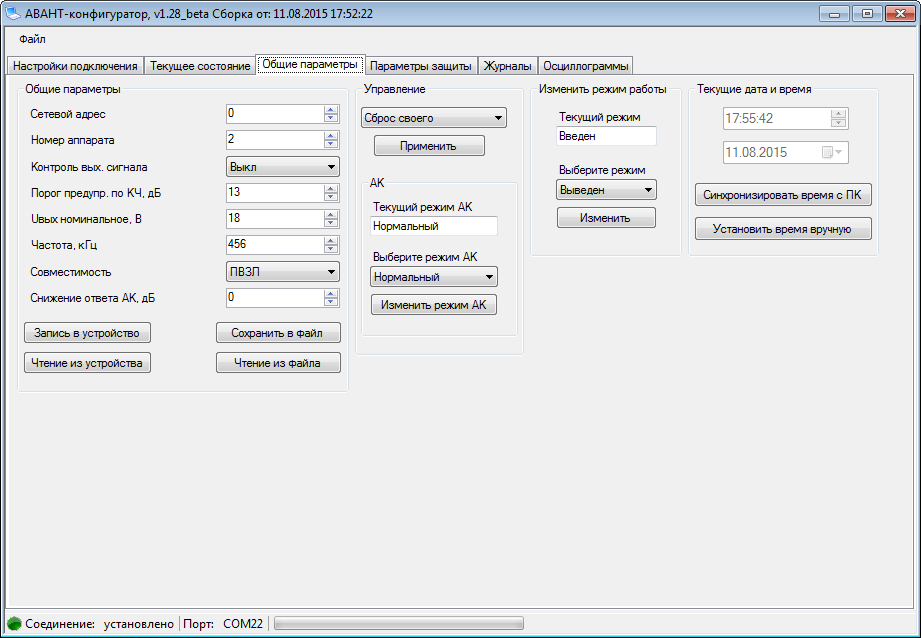
\includegraphics[width=0.8\linewidth]{configurator_param_glb.png}}
	
	\caption{Страница <<Общие параметры>>}
	\label{fig:configurator_param_glb}
\end{figure}


%%% ----------
\subsection{Страница <<Параметры защиты>>}	\label{ssec:configurator_param_def}

На странице <<Параметры защиты>> возможны чтение, изменение и запись в приемопередатчик параметров защиты. Запись параметров осуществляется только в режиме <<Выведен>>.
\newline 

\textbf{Просмотр и изменение параметров защиты}

Для того чтобы просмотреть установленные в настоящее время параметры работы передатчика команд необходимо на панели меню выбрать <<Параметры/Чтение из устройства/Параметры защиты>>. Считанные из приемопередатчика параметры отобразятся в соответствующих полях панели <<Параметры защиты>>.

Для того чтобы изменить параметры, необходимо ввести желаемые значения параметров и выбрать на панели меню <<Параметры/Запись в устройство/Параметры защиты>>. 
\newline 

\textbf{Сохранение и чтение параметров из файла}

Существует возможность сохранить измененные параметры работы приемопередатчика в файл, для этого необходимо на панели меню выбрать <<Параметры/Сохранить в файл>>, в появившемся окне выбрать место для сохранения, ввести имя файла и нажать <<Сохранить>>. В созданный файл будут сохранены все параметры работы приемопередатчика: общие и параметры защиты.

Для того чтобы считать ранее сохраненные параметры из файла необходимо на панели меню выбрать <<Параметры/Загрузить из файла>>, в появившемся окне выбрать файл с параметрами и нажать <<Открыть>>. Из выбранного файла будут считаны все параметры работы приемопередатчика: общие и параметры защиты. 

\begin{figure}[H]
	\center{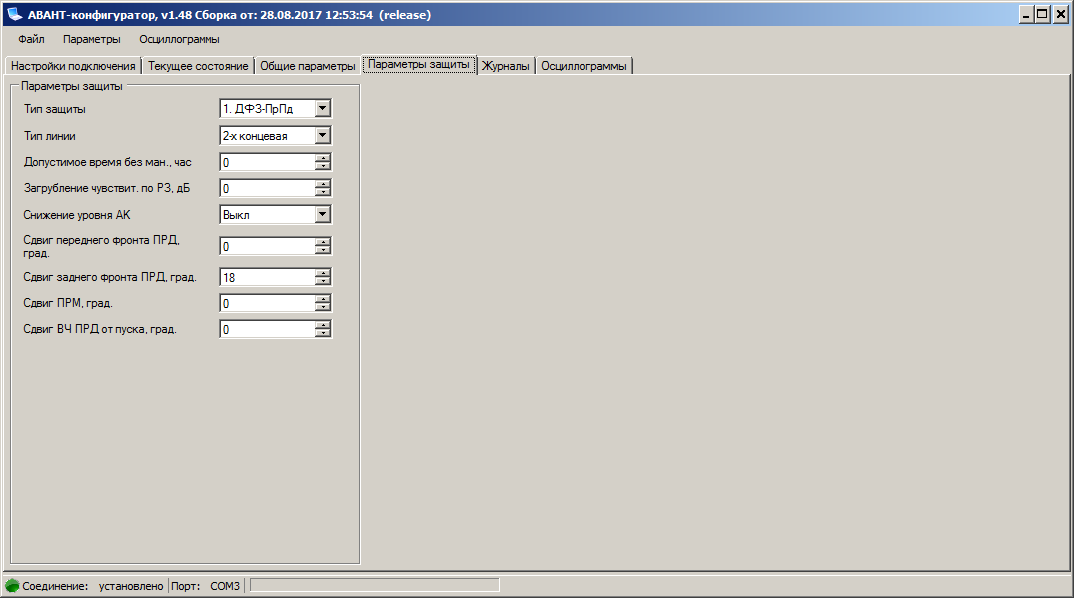
\includegraphics[width=0.8\linewidth]{configurator_param_def.png}}
	
	\caption{Страница <<Параметры защиты>>}
	\label{fig:configurator_param_def}
\end{figure}


%%% ----------
\subsection{Страница <<Журналы>>}	\label{ssec:configurator_journal}

В верхнем левом углу страницы <<Журналы>> расположены две закладки, соответствующие двум различным журналам данных:
\begin{enumerate}
	\item[1.] Журнал событий – журнал общих событий и неисправностей приемопередатчика;
	\item[2.] Журнал защиты – журнал работы приемопередатчика с терминалом защиты: запись управляющих воздействий от терминала (пуск передатчика, останов, манипуляция), запись фактов приема и передачи ВЧ сигналов.
\end{enumerate}

На каждой из страниц журналов расположены:
\begin{enumerate}
	\item[1.] кнопки управления: <<Чтение журнала>>, <<Сохранить в файл>>, <<Загрузить из файла>>;
	\item[2.] строка состояния, в которой отображается название журнала и количество записей в нем;
	\item[3.] таблица с записями журнала.
\end{enumerate}

\begin{figure}[H]
	\center{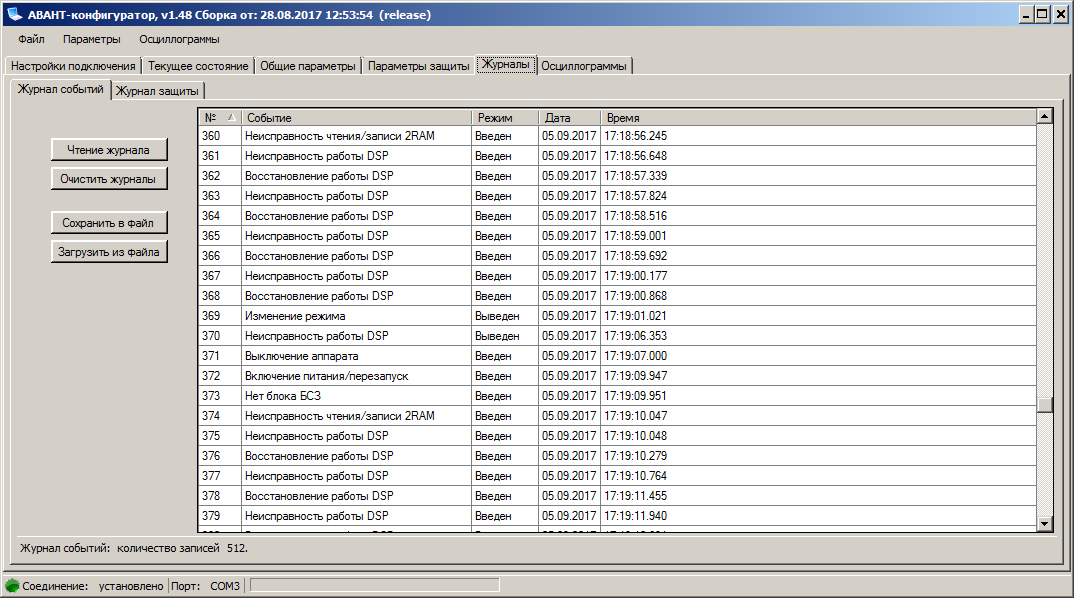
\includegraphics[width=0.9\linewidth]{configurator_journal.png}}
	
	\caption{Страница <<Журналы: События>>}
	\label{fig:configurator_journal}
\end{figure}

\textbf{Чтение журнала}

Для того чтобы считать журнал из приемопередатчика, необходимо нажать на кнопку <<Чтение журнала>>, при этом начнется чтение соответствующего журнала, внизу страницы в строке состояния отобразится количество записей данного журнала. После завершения чтения журнала все записи отобразятся в таблице.

Таблица журнала событий состоит из пяти колонок:
\begin{enumerate}
	\item[1.] № – номер записи;
	\item[2.] Событие – произошедшее событие, неисправность;
	\item[3.] Режим – режим работы приемопередатчика, при котором произошло событие;
	\item[4.] Дата события;
	\item[5.] Время события.
\end{enumerate}

Таблица журнала защиты состоит из десяти колонок:
\begin{enumerate}
	\item[1.] № – номер записи;
	\item[2.] Дата события;
	\item[3.] Время события.
	\item[4.] Состояние – состояние приемопередатчика, при котором произошло событие;
	\item[5.] Пуск – состояние входа Пуск приемопередатчика;
	\item[6.] Останов – состояние входа Останов приемопередатчика;
	\item[7.] Ман – состояние входа манипуляции приемопередатчика;
	\item[8.] ПРД – состояние передатчика: 1~–~передатчик запущен, 0~–~передатчик остановлен;
	\item[9.] ПРМ – состояние приемника: 1~–~приемник принимает сигнал РЗ, 0~–~приемник ничего не принимает;
	\item[10.] Выход приемника – состояние выхода приемника.
\end{enumerate}
	
\textbf{Сохранение и чтение журнала из файла}

Существует возможность сохранить каждый журнал в файл, для этого необходимо нажать на кнопку <<Сохранить в файл>>, в появившемся окне выбрать место для сохранения, ввести имя файла и нажать <<Сохранить>>. В созданный файл будет сохранен соответствующий журнал данных. 

Для того чтобы считать ранее сохраненный журнал из файла, необходимо нажать на кнопку <<Загрузить из файла>>, в появившемся окне выбрать файл с журналом и нажать <<Открыть>>. Из выбранного файла в таблицу конфигуратора будет загружен соответствующий журнал данных.
